\documentclass{beamer}

%% \documentclass[handout]{beamer}
%% % use this with the [handout] option to create handouts for the audience
%% \usepackage{pgfpages}
%% \pgfpagesuselayout{2 on 1}[a4paper,border shrink=5mm]

\mode<presentation>
{
  \usetheme{Diku}
% set this to your preferences:
  \setbeamercovered{invisible}
%  \setbeamercovered{transparent}
}

\usepackage{graphicx}
\usepackage{epic}

\usepackage{amsmath}
\usepackage{amssymb}
\usepackage{amsthm}

\newcommand{\basetop}[1]{\vtop{\vskip-1ex\hbox{#1}}}
\newcommand{\source}[1]{\let\thefootnote\relax\footnotetext{\scriptsize\textcolor{kugray1}{Source: #1}}}

% for coloured code citation in text:
\usepackage{fancyvrb}

%%%%%%%%%%%%%%%%%%%%%%%%%%%%%%%%%
%%%%%    code sections   %%%%%%%%
%%%%%%%%%%%%%%%%%%%%%%%%%%%%%%%%%

% code highlighting commands in own block
\DefineVerbatimEnvironment{code}{Verbatim}{fontsize=\scriptsize}
\DefineVerbatimEnvironment{icode}{Verbatim}{fontsize=\scriptsize}

% Fancy code with color commands:
\DefineVerbatimEnvironment{colorcode}%
        {Verbatim}{fontsize=\scriptsize,commandchars=\\\{\}}

%%%%%%%%%%%%%%%%%%%%%%%%%%%%%%%%%%
%%%%%    some coloring    %%%%%%%%

\definecolor{Red}{RGB}{220,50,10}
\definecolor{Blue}{RGB}{0,51,102}
\definecolor{Yellow}{RGB}{102,51,0}
\definecolor{Orange}{RGB}{178,36,36}
\definecolor{Grey}{RGB}{180,180,180}
\definecolor{Green}{RGB}{20,120,20}
\definecolor{Purple}{RGB}{160,50,100}
\newcommand{\red}[1]{\textcolor{Red}{{#1}}}
\newcommand{\blue}[1]{\textcolor{Blue}{{#1}}}
\newcommand{\yellow}[1]{\textcolor{Yellow}{{#1}}}
\newcommand{\orange}[1]{\textcolor{Orange}{{#1}}}
\newcommand{\grey}[1]{\textcolor{Grey}{{#1}}}
\newcommand{\green}[1]{\textcolor{Green}{{#1}}}
\newcommand{\purple}[1]{\textcolor{Purple}{{#1}}}




% use "DIKU green" from our color theme for \emph
\renewcommand{\emph}[1]{\textcolor{structure}{#1}}
% use some not-too-bright red for an \emp command
\definecolor{DikuRed}{RGB}{130,50,32}
\newcommand{\emp}[1]{\textcolor{DikuRed}{ #1}}
\definecolor{CosGreen}{RGB}{10,100,70}
\newcommand{\emphh}[1]{\textcolor{CosGreen}{ #1}}
\definecolor{CosBlue}{RGB}{55,111,122}
\newcommand{\emphb}[1]{\textcolor{CosBlue}{ #1}}
\definecolor{CosRed}{RGB}{253,1,1}
\newcommand{\empr}[1]{\textcolor{CosRed}{ #1}}

\newcommand{\mymath}[1]{$ #1 $}
\newcommand{\myindx}[1]{_{#1}}
\newcommand{\myindu}[1]{^{#1}}

\newcommand{\Fasto}{\textsc{Fasto}\xspace}


%%%%%%%%%%%%%%%%%%%%

\title[Interconnect]{Scalable Cache Coherence \& Interconnect}

\author[C.~Oancea]{Cosmin E. Oancea {\tt cosmin.oancea@diku.dk}}

\institute{Department of Computer Science (DIKU)\\University of Copenhagen}


\date[Sept 2014]{September 2014 PMPH Lecture Notes}


\begin{document}

\titleslide

\begin{frame}
\frametitle{Structure of a Compiler}

\begin{tabular}{ccc}
Program text&&\\
$\downarrow$ &&\\
\framebox{Lexical analysis} && Binary machine code\\
$\downarrow$ && $\uparrow$ \\
Symbol sequence && \textcolor{gray}{\framebox{Assembly and linking}} \\
$\downarrow$ && $\uparrow$ \\
\framebox{Syntax analysis} && Ditto with named registers\\
$\downarrow$ && $\uparrow$ \\
Syntax tree && \framebox{Register allocation} \\
$\downarrow$ && $\uparrow$ \\
\red{\framebox{Type Checking}} && Symbolic machine code\\
$\downarrow$ &&  $\uparrow$ \\
Syntax tree  && \framebox{Machine code generation} \\
$\downarrow$ && $\uparrow$ \\
\framebox{Intermediate code generation} &$\longrightarrow$ & Intermediate code
\end{tabular}

\end{frame}



%%%%%%%%%%%%%%%%%%%%%%%%%%%%%%%%%%%%%%%%%%%%%%%%%%%%%%%%%%%%%%%%%%%%%%
%%%%%%%%%%%%%%%%%%%%%%%%%%%%%%%%%%%%%%%%%%%%%%%%%%%%%%%%%%%%%%%%%%%%%%
%%%%%%%%%%%%%%%%%%%%%%%%%%%%%%%%%%%%%%%%%%%%%%%%%%%%%%%%%%%%%%%%%%%%%%
\begin{frame}[fragile]
	\tableofcontents
\end{frame}

%%%%%%%%%%%%%%%%%%%%%%%%%%%%%%%%%%%%%%%%%%%%%%%%%%%
%%%%%%%%%%%%%%%%%%%%%%%%%%%%%%%%%%%%%%%%%%%%%%%%%%%
%%%%%%%%%%%%%%%%%%%%%%%%%%%%%%%%%%%%%%%%%%%%%%%%%%%

\section{Scalable Shared Memory Systems}

\begin{frame}[fragile,t]

\begin{columns}
\column{0.66\textwidth}
\frametitle{Typical Memory Hierarchy}
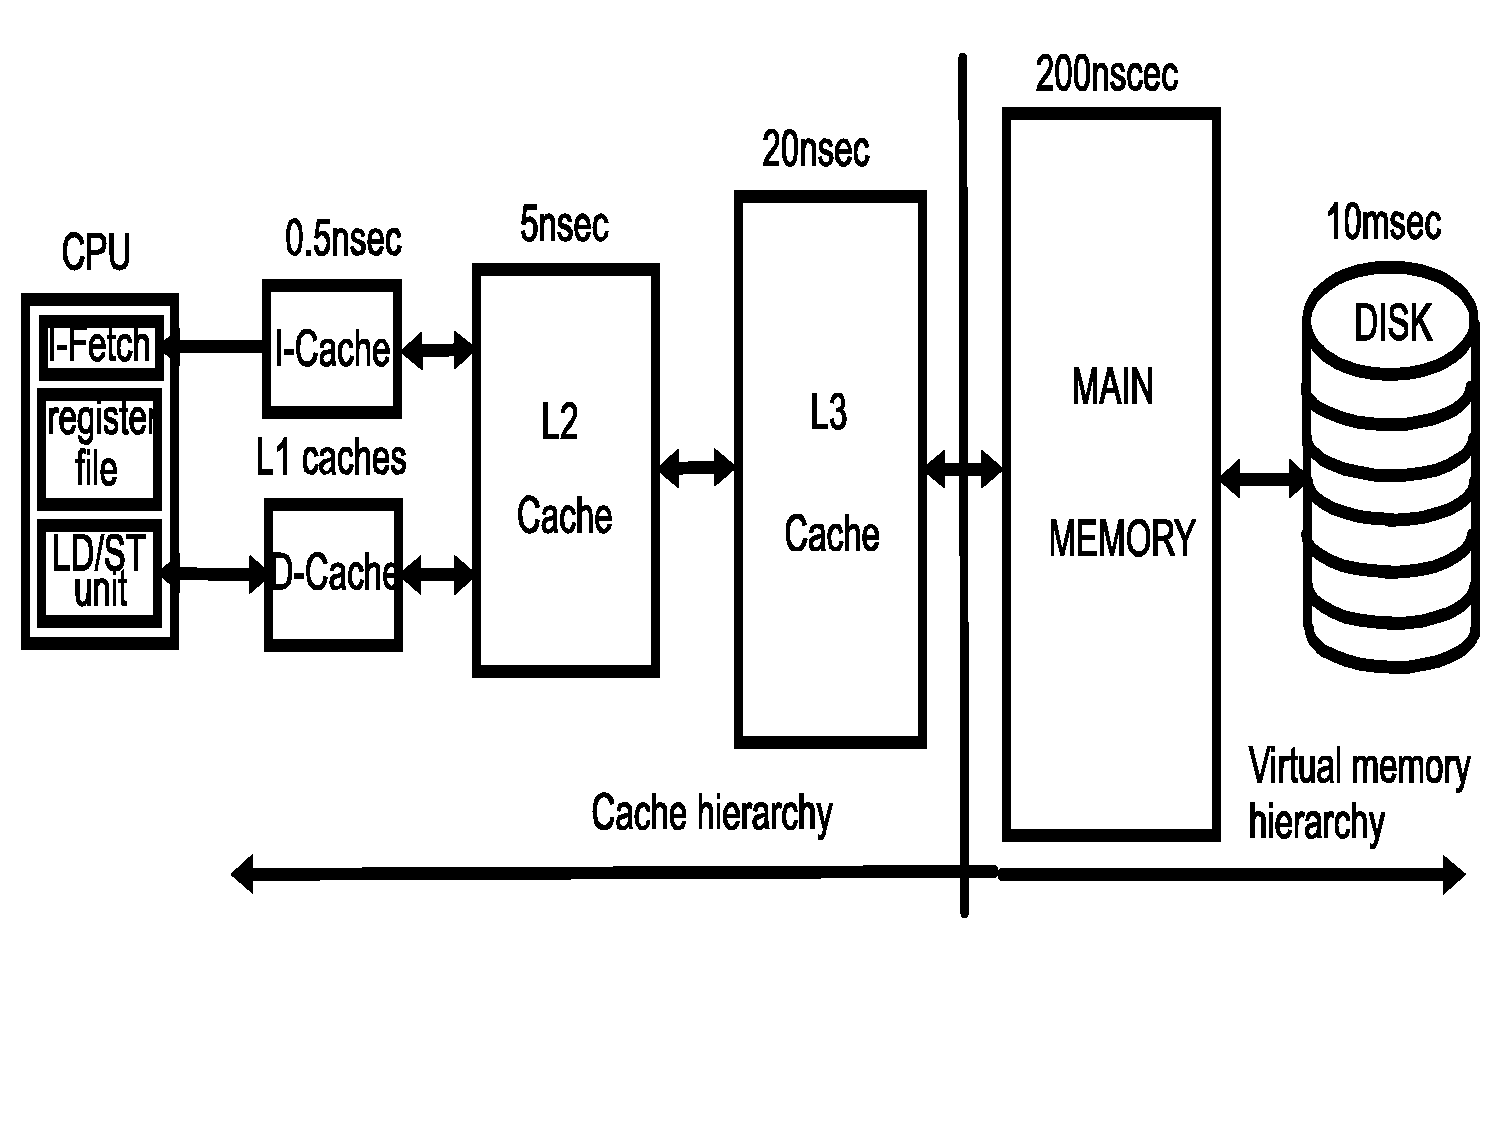
\includegraphics[width=44ex]{FigsMemH/MemHierarchy}
\column{0.30\textwidth}
\emph{Memory goes at electronic speed}, \emp{Disk at mechanical speed.}
\end{columns}
\vspace{-5ex}

\pause
\emph{Locality Principle:}\pause
\begin{itemize}
    \begin{scriptsize}
    \item small set of addresses accessed at a time, 
            named \emph{working set}, $\Rightarrow$ low miss rate,
    \item when program transitions $\Rightarrow$ abrupt change of working sets 
            $\Rightarrow$ high miss rate,
    \item \emph{Temporal Locality:} a referenced item is likely to be accessed again soon,
    \item \emph{Spatial Locality:} items close-by a referenced item likely to be accessed soon,
    \item \emph{Spatial $\Rightarrow$ Temporal} at block/page level.
    \end{scriptsize} 
\end{itemize}
\end{frame}


\end{document}
